\documentclass[a4paper]{article}
\everymath{\displaystyle}
\usepackage{mathtools}
\usepackage{multicol}
\usepackage{tikz}
\usetikzlibrary{decorations.pathmorphing,patterns}
\setlength{\topmargin}{-60pt}
\addtolength{\oddsidemargin}{-80pt}
\addtolength{\evensidemargin}{-80pt}
\addtolength{\textwidth}{160pt}
\addtolength{\textheight}{120pt}
\setlength{\parindent}{0pt}
\setlength{\parskip}{10pt}
\pagenumbering{gobble}
\begin{document}
\section{Fuerza de Rozamiento}
\subsection{Rozamiendo Estático}
Siempre es opesta al movimiento del objeto y paralela a la superficie,
y tiene un módulo máximo de \(
|F_{re}| \le \mu_e \cdot |N|
\), $N =$ normal y $\mu_e$ constante de rozamiento estático. El objeto
comienza a moverse cuando la fuerza sobre él sobrepasa \(\mu_e \cdot |N| \)
\subsection{Rozamiendo Dinámico}
La fuerza está dada por \(
F_{rd} = \mu_d \cdot N
\) con $\mu_d$ el coeficiente de rozamiento dinámico. $F_{rd}$ siempre actúa
contraria al desplazamiento.

Se tiene \(
	0 \le \mu_d \le \mu_e \le 1
\)
\section{Movimiento Circular}
Se tiene \(
a_c = \frac{V^2}{R} = \omega^2R
\), $a =$ aceleración centrípeta, $V$ velocidad y $\omega$ velocidad angular
\section{Péndulo Cónico}
Actúa sobre la masa la tensión $T$ y el peso $P$, si el ángulo del hilo con
la vertical es $\alpha$ tenemos:
\[
	T_y + P = 0 \iff T_y = -P \text{, y}
\]
\[
	T_x = F_c = m \cdot a_c = m \cdot \omega^2 \cdot R
\]
donde $R$ = $\ell \cdot \sin \alpha$, $T_x = T \cdot \sin \alpha$ y $T_y
= T \cdot \cos \alpha$
\section{Peralte}
Sobre el auto actúan la normal ($N$), el peso ($P$),
y el rozamiento $F_{re}$.
Se ponen los ejes alineados con el piso, y se tiene:

\begin{multicols}{3}
	$\quad$
	\columnbreak

\begin{tikzpicture}
	\draw (0,0) -- (4,0) -- (0, 2) -- cycle;
	\draw (2, 1.5) circle (0.45cm);
	\draw[thick,->] (2, 1.5) -- (2, 0.5) node[anchor=east]{P};
	\draw[thick,->] (2, 1.5) -- (3, 1) node[anchor=west]{$F_{re}$};
	\draw[thick,->] (2, 1.5) -- (2.8, 3.1) node[anchor=west]{N};
	\draw[thick,->] (2, 1.5) -- (4, 1.5) node[anchor=west]{$F_c$};
\end{tikzpicture}
\columnbreak

\[\quad\]
\(
	N_x + F_{rex}  = F_c = ma_c
\)
\[\quad\]
\(
	N_y - F_{rey} - P = 0
\)
\end{multicols}
\section{Gravitación}
La fuerza de gravitación entre dos objetos de masa $m$ y $M$ con
distancia entre centros $r$ está dada por \(
F_g = G\frac{mM}{r^2}
\)
En una órbita se tiene $m(a_c = \omega^2r) = G\frac{mM}{r^2} \iff
\omega^2r^3 = GM$, donde $M$ es la masa del objeto mayor (alrededor del cual
se orbita).
\(\text{La constante de gravitación es } G = 6.67 \cdot 10^{-11}
Nm^2kg^{-2}\)

\section{Fuerzas Elásticas}
Ley de Hooke $F_e = K\cdot \Delta\ell$, donde $\Delta\ell = \ell - \ell_0$,
con $\ell_0$ la longitud natural del resorte.
\begin{multicols}{2}

	\subsection{Resortes en paralelo}
\begin{tikzpicture}
	\draw[decoration={segment length=1.5mm,coil},decorate] (0,0) -- (2,0);
	\draw[decoration={segment length=2.5mm,coil},decorate] (0,0.5) -- (2,0.5);
\end{tikzpicture}

\[
F_e = F_{e1} = F_{e2}
\]
\[
\Delta\ell = \Delta\ell_1 + \Delta\ell_2
\]
\[
	k = \frac{1}{\frac{1}{k_1} +\frac{1}{k_2}}
\]

	\columnbreak

	\subsection{Resortes en serie}
\begin{tikzpicture}
	\draw[decoration={segment length=1.5mm,coil},decorate] (0,0) -- (1,0);
	\draw[decoration={segment length=2.5mm,coil},decorate] (1,0) -- (3,0);
\end{tikzpicture}

\[
F_e = F_{e1} + F_{e2}
\]
\[
\Delta\ell = \Delta\ell_1 = \Delta\ell_2
\]
\[
	k = k_1 + k_2
\]
\end{multicols}
\section{Estática de Cuerpo Puntual}
Hacemos DCL y usamos $\sum F_x = \sum F_y = 0$ (estableciendo primero un
buen marco de referencia).

\section{Estática de Cuerpo Extenso}
Tenemos $\sum F_x = \sum F_y = \sum M_O$ para algún marco de referencia
arbitrario y algún centro de rotación $O$

$M_O[Nm]$ se calcula dada una fuerza $F$ sobre un punto $P$, como $(O - P)
\times F$, osea es la componente de $F$ perpendicular a $PO$, el signo dado
con la regla de la mano derecha.
\section{Hidrostática}
\(
	760\;torr = 760\;mmHg = 1\;atm = 101\,325\;Pa
\), con \(
Pa = Nm^{-2}
\)

La presión absoluta está dada por $P_{abs} = P_{atm} + \rho gh$, y la
relativa por $P_{rel} = \rho gh$, deonde $\rho$ es la densidad del fluido
$\left(\rho = \frac{m}{Vol}, [\rho] = \frac{kg}{m^3}\right)$, $g =
10ms^{-2}$ es la gravedad y $h$ es la profundidad del punto que se mide
(desde la superficie)
\subsection{Gas Ideal}
se tiene $PV = nRT$, osea que la presión $P$ no depende de la altura como el
el líquido, y es constante en todo el gas.
\subsection{Principio de Pascal}
Si cambia la presión el angún punto, cambia en todos
\subsection{Principio de Igual Presión $-$ Igual Altura}
se tiene $P_a = P_b$ para cualesquiera dos puntos $a$, $b$ de la misma
componente conexa de un mismo líquido y que estén a la misma altura.
\end{document}
